\documentclass[a4paper,12pt]{report} % добавить leqno в [] для нумерации слева

%%% Работа с русским языком
\usepackage{cmap}					% поиск в PDF
\usepackage{mathtext} 				% русские буквы в формулах
\usepackage[T2A]{fontenc}			% кодировка
\usepackage[utf8]{inputenc}			% кодировка исходного текста
\usepackage[english,russian]{babel}	% локализация и переносы

%%% Дополнительная работа с математикой
\usepackage{amsmath,amsfonts,amssymb,amsthm,mathtools} % AMS
\usepackage{icomma} % "Умная" запятая: $0,2$ --- число, $0, 2$ --- перечисление

%% Номера формул
\mathtoolsset{showonlyrefs=true} % Показывать номера только у тех формул, на которые есть \eqref{} в тексте.

%% Шрифты
\usepackage{euscript}	 % Шрифт Евклид
\usepackage{mathrsfs} % Красивый матшрифт

%% Свои команды
\DeclareMathOperator{\sgn}{\mathop{sgn}}

%\setlength\parindent{0ex}
%\setlength\parskip{0.3cm}

%%% Заголовок
\author{Волков Павел А-14-19}
\title{Типовой расчет №2 по численным методам Вариант 3}
\date{\today}

\usepackage{graphicx}

\begin{document} % конец преамбулы, начало документа

\maketitle

\newpage
\section*{Задание}
Локализовать корень нелинейного уравнения $f(x) = 0$ и найти его методом бисекции с точностью $\varepsilon = 0.01$
\[
    f(x) = x^2 - 3x - \frac{1}{x + 1}
\]

\section*{Решение}

\subsection*{Локализация корней}
Построим график функции $f(x) = x^2 - 3x - \frac{1}{x + 1}$

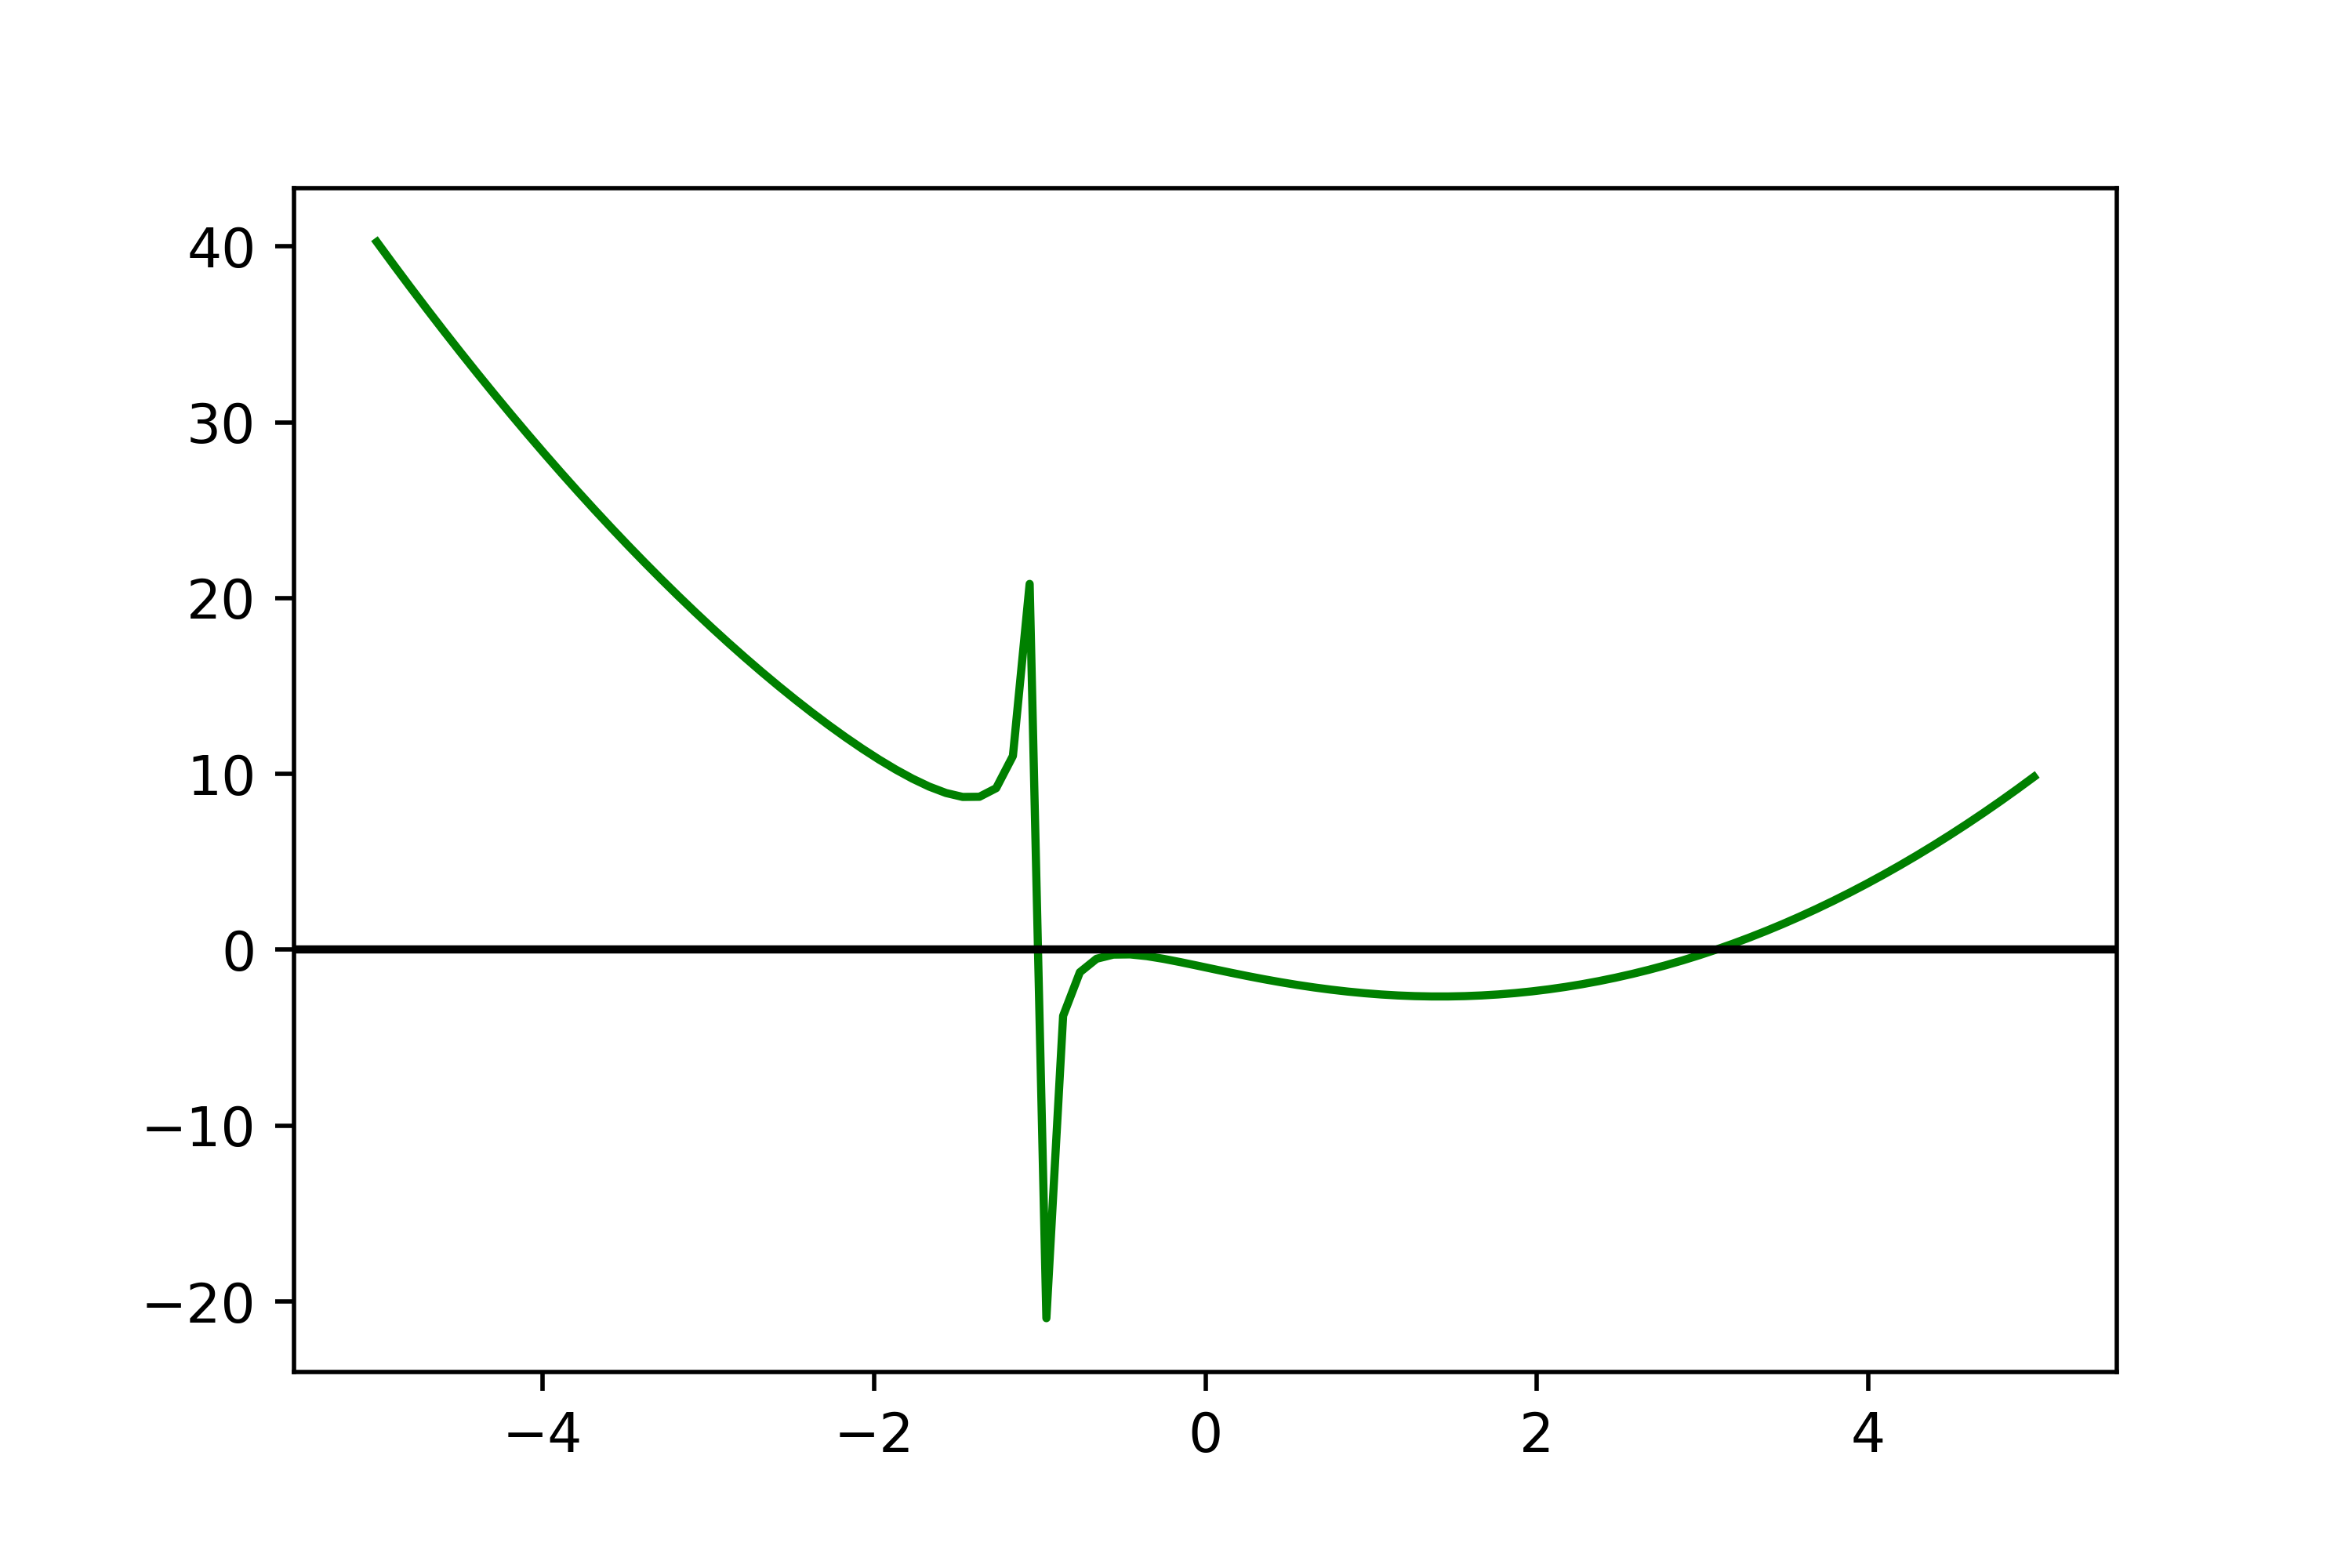
\includegraphics{func_plot.png}

Таким образом, отрезок локализации - $[2, 4]$
Действительно, $f(2) = -2.333; f(4) = 3.8$

Найдем производную $f'(x) = 2x - 3 + \frac{1}{(x+1)^2} > 0 ~ \forall x \geq 2$ - следовательно на данном отрезке существует только один корень

\newpage
\subsection*{Применение метода}
Все шаги каждой итерации представлены в таблице ниже:

\begin{tabular}{ | c | c | c | c | c | c | c |}
    \hline
    $k$ & $a^{(k)}$ & $x^{(k)}$ & $b^{(k)}$ & $f(a^{(k)})$ & $f(x^{(k)})$ &  $b^{(k)}$ - $a^{(k)}$\\ \hline
    0 & 2 & 3 & 4 & -2.333333 & -0.25 & 2 \\ \hline
    1 & 3 & 3.5 & 4 & -0.25 & 1.527778 & 1  \\ \hline
    2 & 3 & 3.25 & 3.5 & -0.25 & 0.577206 & 0.5\\ \hline
    3 & 3 & 3.125 & 3.25 & -0.25 & 0.148201 & 0.25 \\ \hline
    4 & 3 & 3.0625 & 3.125 & -0.25 & -0.054748 & 0.125 \\ \hline
    5 & 3.0625 & 3.09375 & 3.125 & -0.054748 & 0.045764 & 0.0625 \\ \hline
    6 & 3.0625 & 3.078125 & 3.09375 & -0.054748 & -0.004732 & 0.03125 \\ \hline
    7 & 3.078125 & 3.0859375 & 3.09375 & -0.004732 & 0.020456 & 0.015625 \\ \hline

\end{tabular}

На 7-ом шаге длина очередного отрезка стала меньше чем $2\varepsilon$,
то на нем работа метода прекращается и середину последнего отрезка
следует принять за приближенное значение корня.

Ответ: $\overline{x} = x^{(7)} \pm \varepsilon = 3.09 \pm 0.01$
\end{document}